\chapter{Androidアプリ「LEDOXEA」}
\label{chap:ledoxea}

本章では、開発したAndroidアプリ「LEDOXEA」の利用方法と、その特徴について説明する。

\section{使用方法}
起動後、上部にある検索ボックスから、検索したいキーワードを入力する。入力が完了したら、右側の検索ボタンを押下する。すると検索が行われ、合計5本のラインが画面上に出現する。これらを上下にスワイプすると、検索結果の上下移動が可能であり、ひとつひとつ項目を参照することが可能である。また、別のコンテンツを参照したい時は、左右にスワイプすると回転ハンガーのようにコンテンツが回転し、別のコンテンツが中央に移動する。
\begin{figure}[htbp]
\begin{center}
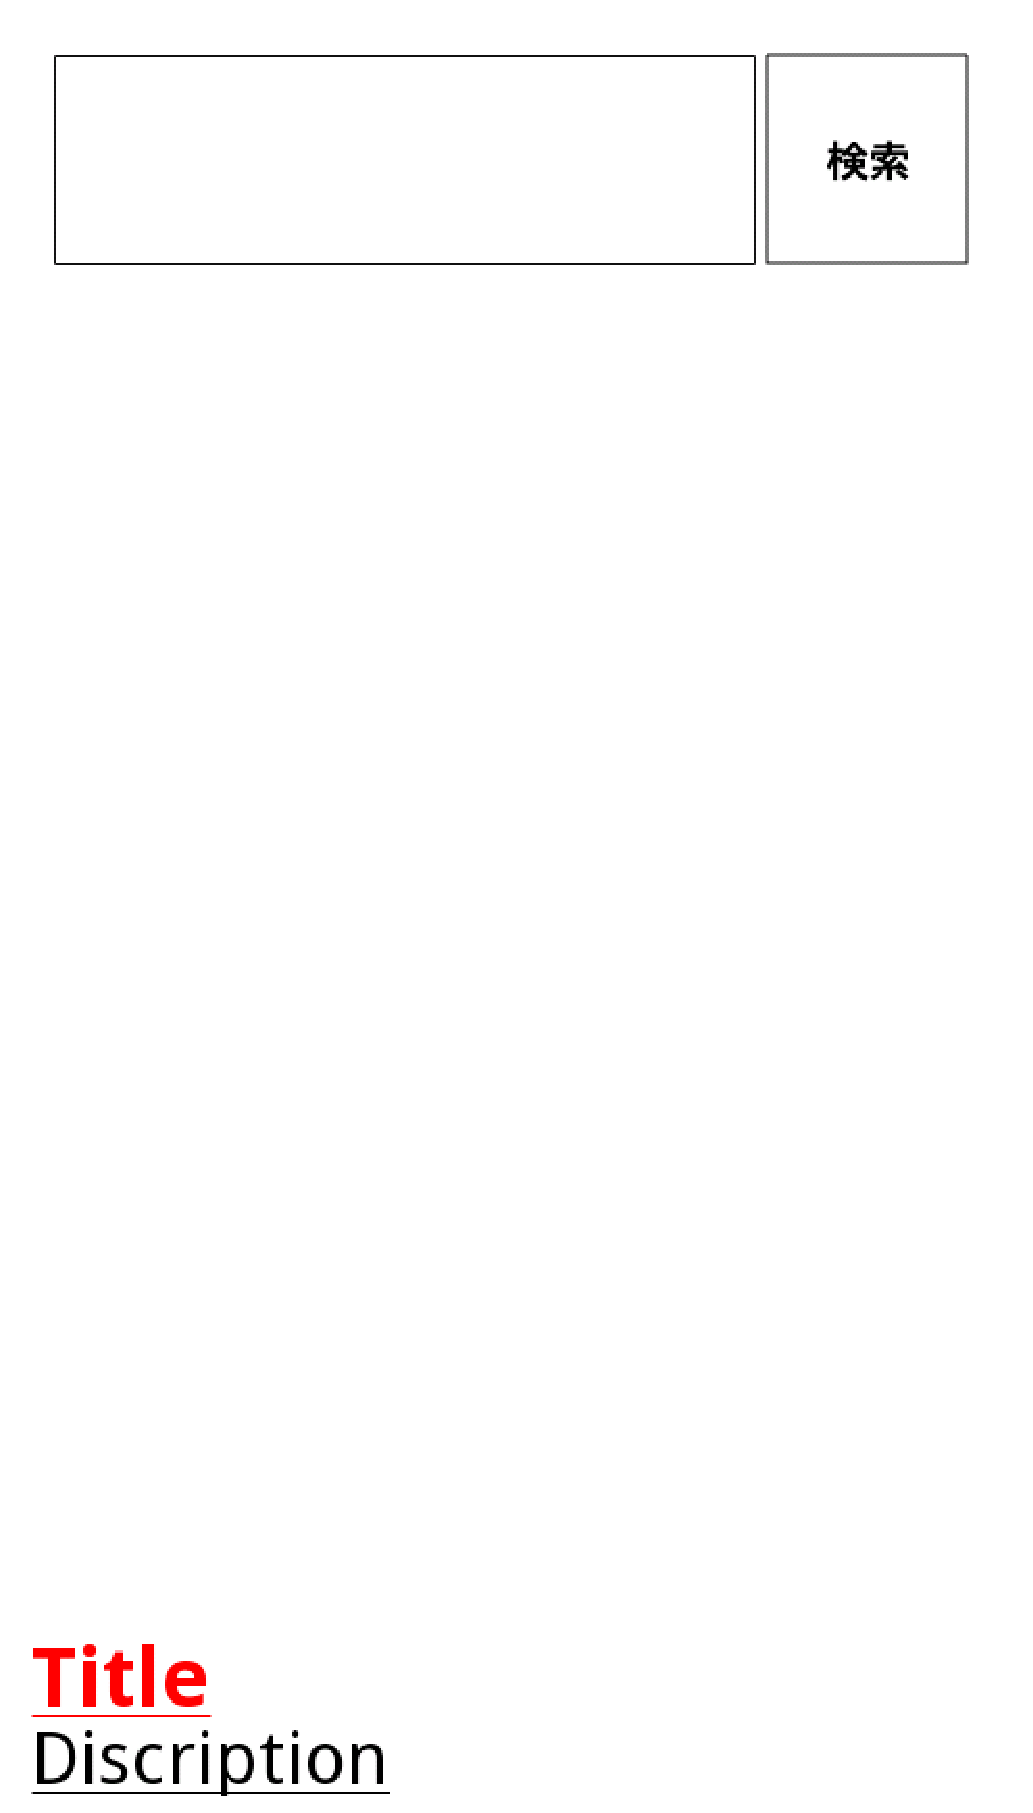
\includegraphics[width=7cm]{le01.eps}
\caption{起動画面}
\label{le01}
\end{center}
\end{figure}

\begin{figure}[htbp]
\begin{center}
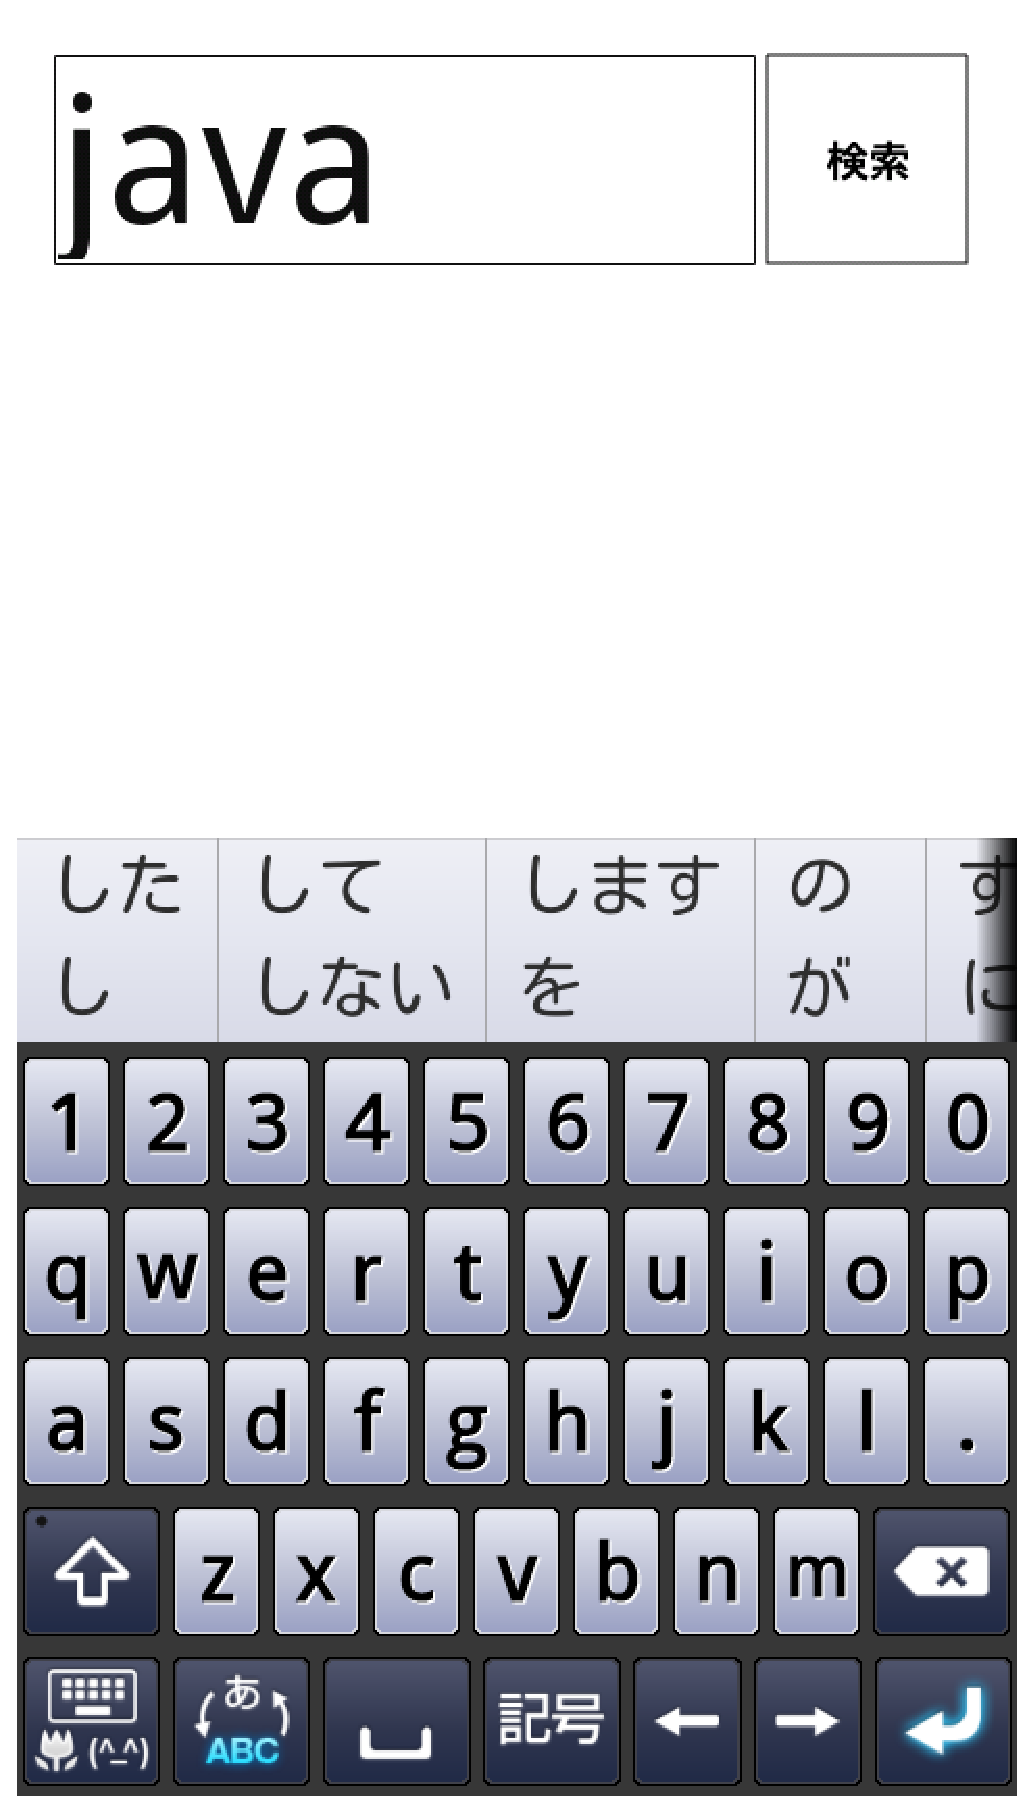
\includegraphics[width=7cm]{le02.eps}
\caption{検索キーワードを入力}
\label{le02}
\end{center}
\end{figure}

\begin{figure}[htbp]
\begin{center}
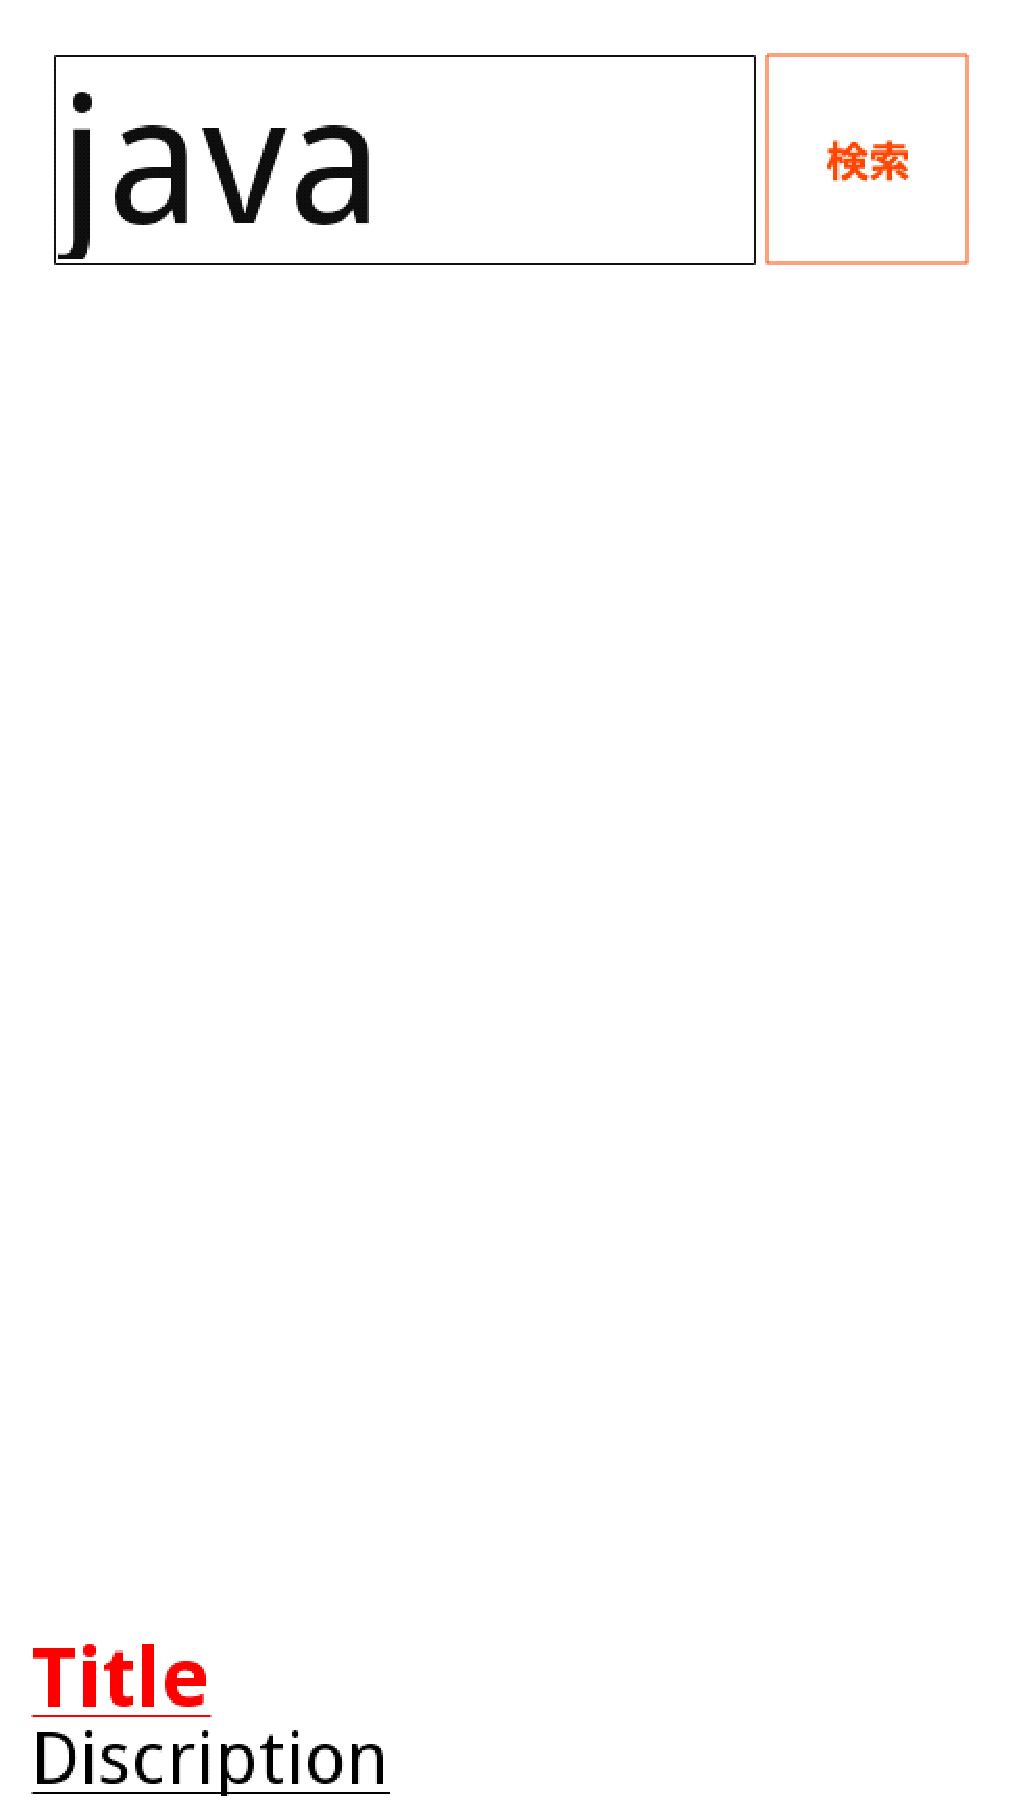
\includegraphics[width=7cm]{le03.eps}
\caption{検索ボタンを押下}
\label{le03}
\end{center}
\end{figure}

\begin{figure}[htbp]
\begin{center}
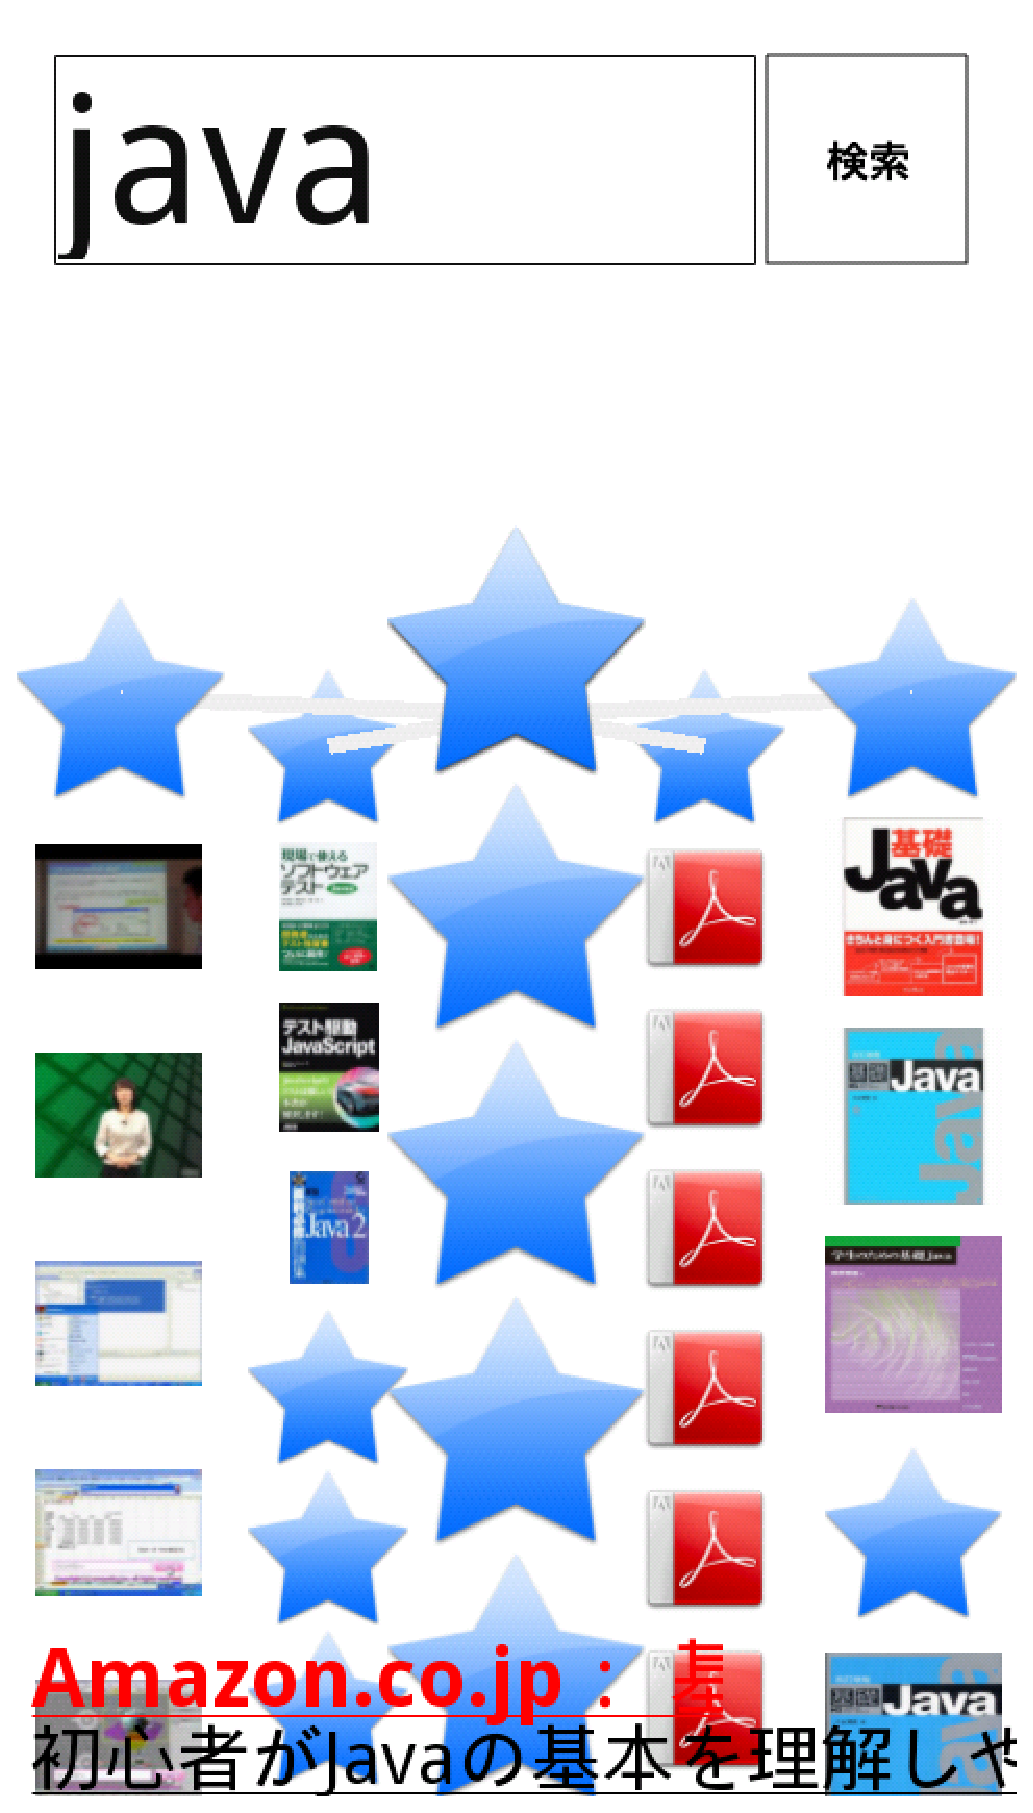
\includegraphics[width=7cm]{le04.eps}
\caption{コンテンツ表示}
\label{le04}
\end{center}
\end{figure}

\begin{figure}[htbp]
\begin{center}
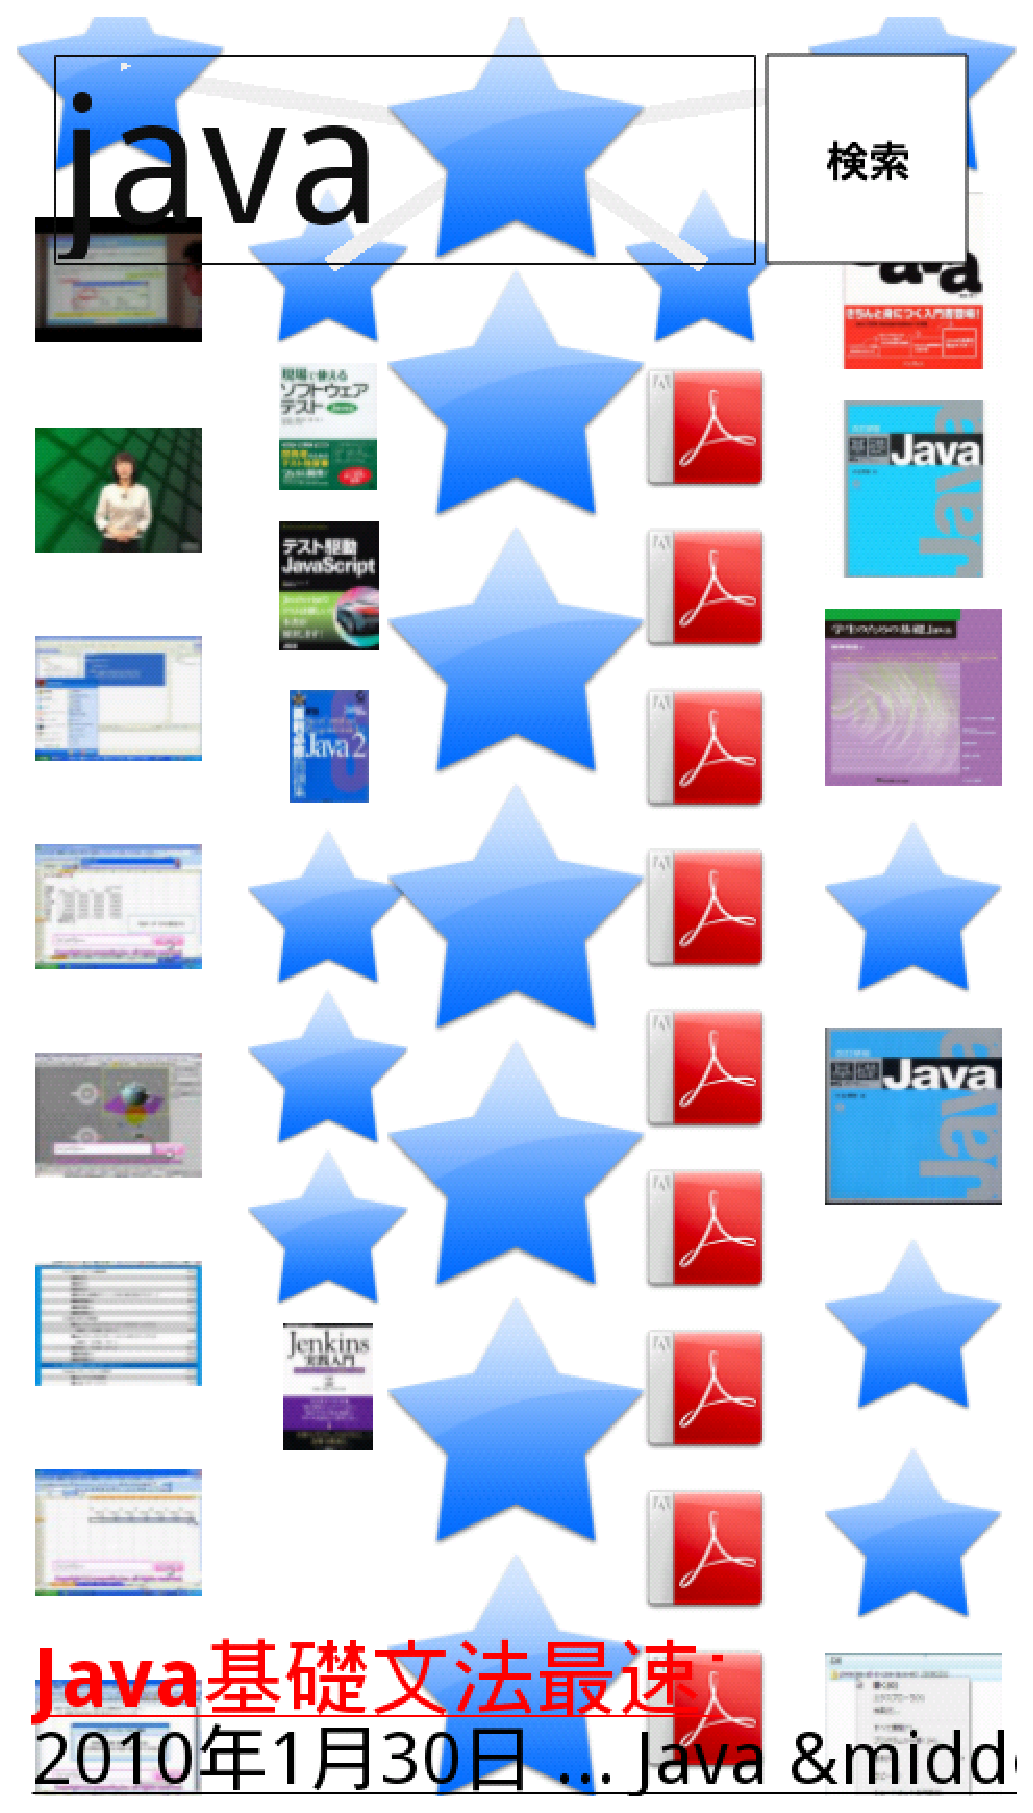
\includegraphics[width=7cm]{le05.eps}
\caption{上にスワイプすることでコンテンツを下に見ていくことが可能}
\label{le05}
\end{center}
\end{figure}

\begin{figure}[htbp]
\begin{center}
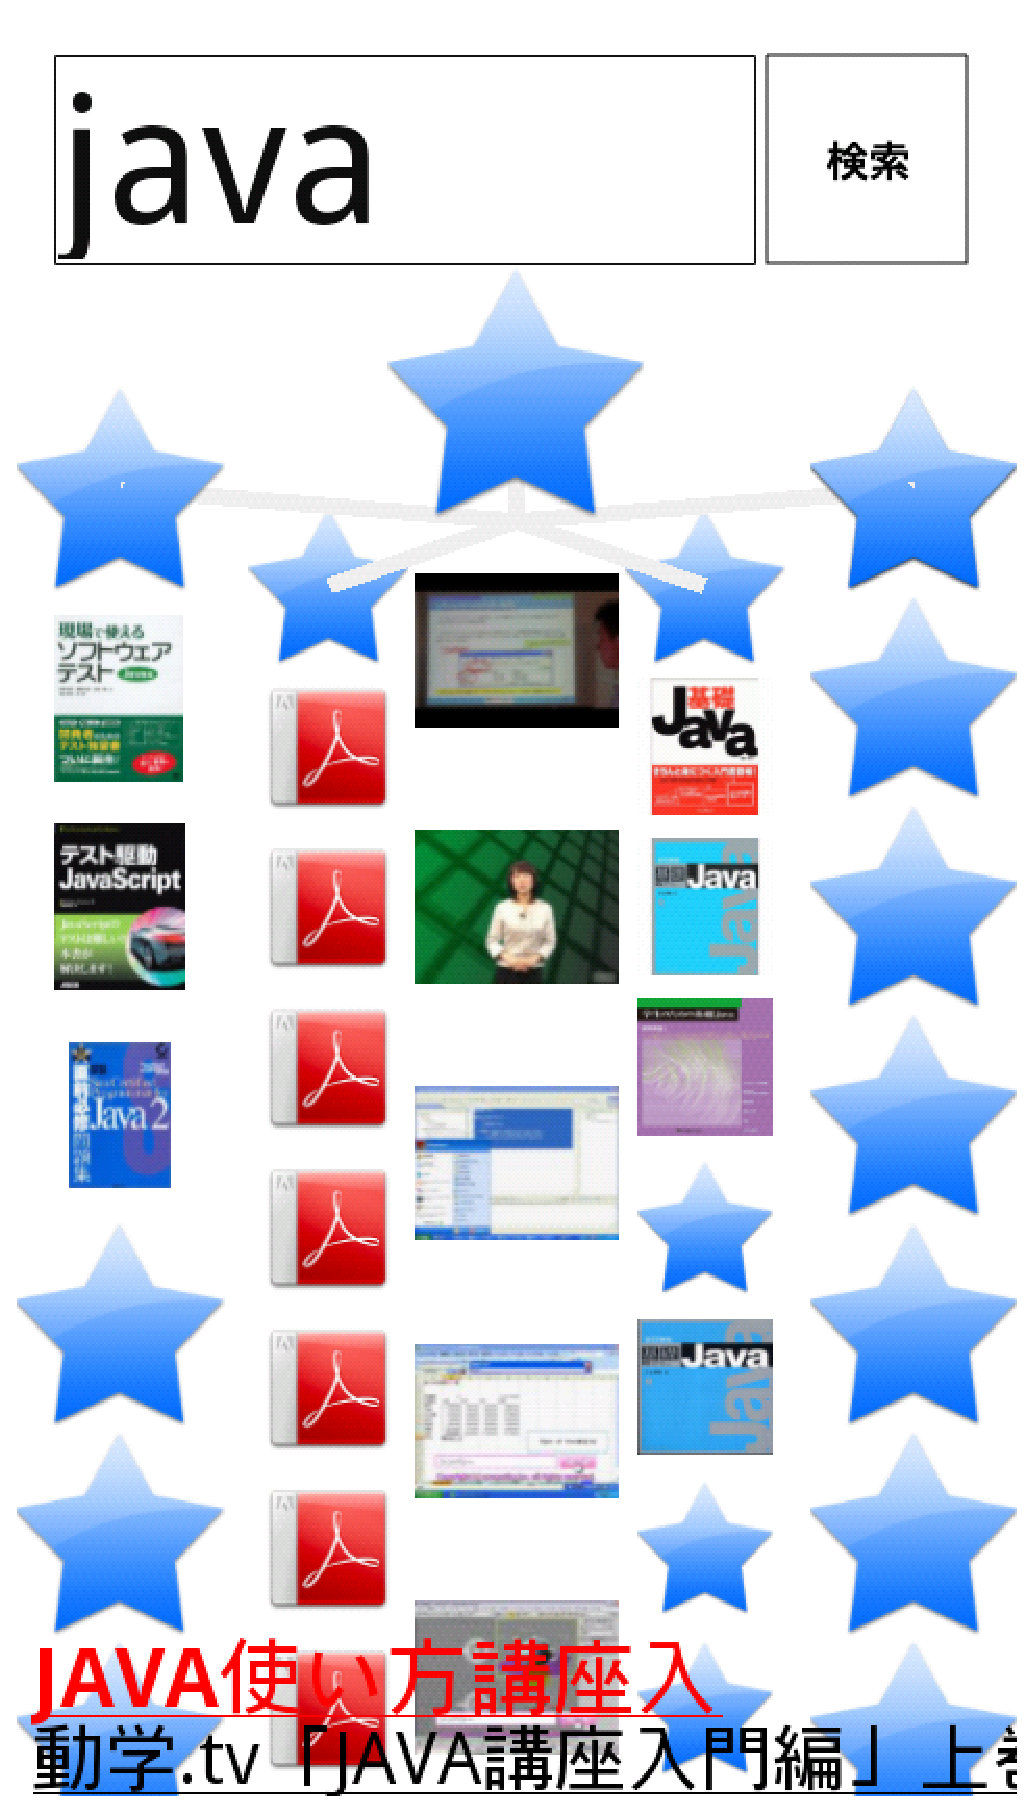
\includegraphics[width=7cm]{le06.eps}
\caption{横にスワイプすることでコンテンツが回転}
\label{le06}
\end{center}
\end{figure}

\section{特徴}
それぞれ実現することができた、特徴について記述する。

\subsection{移植性}
ADOBE AIR の移植性の高さにより、Androidに留まらず、iOS、PCのWebブラウザ、PCアプリケーションとして様々な形態に対応できる。

\subsection{スペック性能への非依存性}
非常に簡易な3次元CGにより製作されているため、60fps程度の安定した高速描画を実現している。

\subsection{フリック操作による直感的操作性}
検索結果を上下や左右に移動するのは直感的に理解しやすく、項目を確認する際に発生する苦痛を軽減することに役立つ。

\subsection{検索エンジンの同時検索、WWW視覚化}
e-learningコンテンツを複数の検索エンジンで同時に高精度で検索できるため、一度の検索で非常に多量の収穫を得ることをできる。